%% main.tex — "Bundling or Silence" (Paper 1), regenerated 2026-07-23 from
%% research/swarm/PAPER-DRAFT.md after the founder revision pass (abstract
%% rewrite, physically-grounded vocabulary, swarm audit, lighter
%% registration narration, global compression). Submission-notes section
%% deliberately excluded; it stays in the markdown.
%%
%% CLASS NOTE: \documentclass[sigconf]{acmart} is a STAND-IN for the official
%% AAMAS/IFAAMAS class. Swap to the ifaamas style file at submission time and
%% re-check all floats/line breaks. [nonacm] suppresses ACM-specific footer
%% boilerplate while drafting.

\documentclass[sigconf,nonacm]{acmart}

\usepackage{booktabs}
\graphicspath{{../figures/}}

\settopmatter{printacmref=false}

%% Layout-quality pass (2026-07-23): no content changes.
%% - \emergencystretch lets TeX loosen interword spacing instead of
%%   emitting overfull lines (long inline code strings were crossing the
%%   column gutter and overlapping the neighboring column).
%% - \raggedbottom stops column-balancing from stretching vboxes into
%%   overlaps ("Underfull \vbox while \output is active").
%% - URL/path break setup: long identifiers (repo URL, sweep artifact
%%   names, engine primitives) are set with \path{} so they can break at
%%   /, -, ., and _ instead of overflowing.
\emergencystretch=3em
\raggedbottom
\expandafter\def\expandafter\UrlBreaks\expandafter{\UrlBreaks\do\_\do\-\do\.\do\/}

\begin{document}

\title{Bundling or Silence: A Pre-Registered Benchmark of Multi-Issue Nash
Bargaining in Mixed-Ownership Robot Fleets}

% Author block filled by founder 2026-07-23.
\author{Santiago Munoz}
\affiliation{%
  \institution{SNHP Research}
  \city{}
  \country{}}
\email{ryuxik@gmail.com}
\renewcommand{\shortauthors}{Munoz}

\begin{abstract}
Twenty-four robots owned by different parties mine ore and haul it to a
sink in a deterministic gridworld, under battery budgets, lossy energy
transfer, and a fixed horizon. Robots can strike bundled deals trading
energy, cargo, and territory claims. Owners differ, so every deal must be
individually rational (IR): no side accepts a loss. We benchmark
Nash-bargained bundles against altruistic rescue, bilateral and broadcast
sequential single-item (SSI) auctions, and a cooperative ceiling, under a
mean-preserving heterogeneity dial. Three claims were registered before
results. C1: single-issue IR trade is structurally infeasible --- only
bundles trade. C2: bargaining with a rescue floor out-delivers the
bilateral auction on two geometries; against the strong SSI baseline a
registered kill fired --- bargaining buys survival, not throughput. C3: the
bargaining$-$auction gap grows with heterogeneity, then saturates. On
moving fields, auction coverage out-explores bargaining; a map-information
market improves audit integrity, not output. Our first registration failed
hostile review; every fired kill is reported.
\end{abstract}

\keywords{multi-robot systems, market-based coordination, multi-issue
negotiation, Nash bargaining solution, pre-registration, benchmark}

\maketitle

\section{Introduction}\label{sec:intro}

Robot deployments increasingly cross ownership boundaries: delivery fleets
in facilities owned by others, robots from different vendors sharing
chargers, mixed fleets in one warehouse. This is commercial practice, not a
hypothetical --- robots-as-a-service contracts already price physical work
per outcome (AutoStore bills warehouse picks per
pick,\footnote{\path{autostoresystem.com/insights/buying-vs-raas-whats-the-best-strategy-for-investing-in-warehouse-robotics}, accessed 2026-07.}
and GXO pays Agility Robotics for humanoid labor by
utilization\footnote{\path{investors.gxo.com/news-releases/news-release-details/gxo-signs-industry-first-multi-year-agreement-agility-robotics}, accessed 2026-07.})
--- so a coordination step between robots with different owners is also a
commercial event between firms. The standard premise of multi-robot
coordination --- one shared objective --- is then false by construction. Each robot answers to its owner, and any step that leaves an
owner worse off will eventually be disabled. Coordination must be
\emph{individually rational} (IR): no participant accepts a loss.

The market-based multi-robot lineage
\cite{gerkey2002murdoch,gerkey2004taxonomy,dias2006market} saw this early
and imported the auction: tasks are announced, robots bid, the cheapest
capable robot wins. But a bid is one scalar. It cannot express the deal
mixed-ownership logistics needs --- ``I take your two crates because I am
efficient and you are nearly dead; you top up my charge and cede your claim
on the near source.'' Multi-issue negotiation (logrolling) is mature in the
automated negotiation community \cite{baarslag2015anac,aydogan2026anac},
yet an adversarially verified literature sweep
(Section~\ref{sec:related}) found no published system in which robots
strike bundled multi-issue agreements with each other.

This paper contributes a benchmark, not a deployment: a controlled world in
which the bargaining layer's value can be isolated, measured, and killed.
Three registered questions: is bundling \emph{necessary} for IR trade (C1)?
How much of the cooperative ceiling does bundled Nash bargaining recover
--- the residual being the \emph{coordination gap} (C2)? Does the advantage
over single-issue auctions grow with heterogeneity (C3)?

Two objections deserve pre-emption. First, with known utilities the Nash
bargaining solution is a computation, not a protocol; the benchmark
therefore treats information quality as a variable, and under estimation
error and lies (v5--v7) the mechanism's measured value is \emph{deal
integrity} --- the true-loss veto turns error into failed proposals --- not
cleverness. Second, our agents are simulated too; what separates them from
the negotiation literature's is not hardware but where utilities come from.
Issue values are computed by executing the candidate deal in the world's
dynamics --- movement costs, the 25\% transfer loss, time-consuming
exchanges, stranding --- not drawn from exogenous preference tables; hence
the evaluated-$\Phi$==executed-$\Phi$ assertion on every deal. We call this
\emph{physically grounded}.

Positioning: this is market-based multi-robot / MAS work, not swarm
robotics --- $N{=}24$, full-information utilities, and a deterministic
gridworld fail the field's own criteria for ``swarm'' \cite{sahin2005swarm},
and we use the word only to say so. All claims were pre-registered with
explicit kill conditions before results --- including a v1 registration
that failed hostile review and was discarded
(Section~\ref{sec:registration}) --- and fired kills are reported as
results, not buried.

\section{Related Work}\label{sec:related}

This section follows an adversarially verified prior-art map (20 primary
sources fetched; 25 claims checked by 3-vote panels: 23 confirmed 3-0, 2
refuted; \texttt{LITERATURE.md} in the code release). Its verdict: the
intersection of multi-issue negotiation and inter-robot coordination is
unoccupied.

\paragraph{Market-based multi-robot coordination is single-issue.}
MURDOCH \cite{gerkey2002murdoch} assigns tasks by first-price one-round
auctions; a bid is one scalar fitness value. TraderBots
\cite{zlot2006auction} extends auctions to task trees, but a bid remains
task + price + tree --- a full-text search of the thesis (187~pp.) finds no
Nash, logrolling, multi-issue, bargaining, or energy exchange. The MRTA
taxonomy \cite{gerkey2004taxonomy} and the Dias et al.\ survey
\cite{dias2006market} frame the field's mechanisms; none bundle issues.
Later robotics ``negotiation'' stays single-issue: task reallocation
\cite{cui2013game}; opponent-utility modeling for task allocation
\cite{ke2012task}.

\paragraph{Multi-issue IR contracting among self-interested agents is not
new.} Sandholm's contract types \cite{sandholm1998contract} give
self-interested agents \emph{cluster} (bundle) contracts, \emph{swaps}, and
multi-agent contracts with side payments under IR; each escapes local
optima the others cannot, and atomic OCSM contracts reach the global
optimum in theory. Andersson and Sandholm \cite{andersson1999sequencing}
sequence contract types for anytime reallocation. Multiagent resource
allocation (MARA) covers the same ground over abstract goods: Chevaleyre et
al.\ \cite{chevaleyre2006mara} survey allocation by negotiation; Endriss et
al.\ \cite{endriss2006negotiating} characterize the deal classes ---
including multilateral bundle deals --- needed for socially optimal
allocations under IR. Our absence claim is therefore narrow: missing is a
\emph{physically grounded} instantiation with \emph{heterogeneous physical
issue types} --- lossy energy vs cargo vs claim rights, each with its own
dynamics --- under \emph{executed dynamics}, benchmarked empirically rather
than proved as reachability results. That gap is the one this benchmark
occupies.

\paragraph{Two terminology traps.} \emph{Combinatorial bids are not
multi-issue deals}: Lin and Zheng \cite{lin2005combinatorial} auction
bundles of \emph{tasks} at one scalar price per bundle --- one issue type,
no cross-issue trade-off. \emph{Nash equilibrium is not Nash bargaining}: a
2025 EAAI paper \cite{hamidoglu2025nash} applies Nash \emph{equilibrium}
analysis to a non-cooperative task-selection game --- no offers, no deals,
no exchange; energy sits inside each robot's own utility. From the other
direction, the 2026 line applying the Nash bargaining solution to
vehicle-to-vehicle energy markets (e.g., arXiv:2605.22363) bargains one
issue --- price/quantity of energy --- over purely economic utilities.
Keyword searches (``combinatorial,'' ``Nash, robots, energy'') wrongly
suggest the niche is occupied.

\paragraph{Robot-robot energy exchange exists in hardware, but is
rule-based.} The CISSBot line demonstrates physical battery swapping
\cite{schioler2008trophallaxis} under Ngo and Schi{\o}ler's probabilistic
``randomized trophallaxis'' \cite{ngo2007randomized} --- no offer or
acceptance step. Moonjaita et al.\ \cite{moonjaita2018trophallaxis} fix
roles by battery thresholds and amounts by energy averaging: numerically an
egalitarian split, no agreement struck. Virtual trophallaxis
\cite{schmickl2008trophallaxis} couples energy to navigation as signaling.
The physical channel our benchmark abstracts exists; the bargaining layer
above it does not.

\paragraph{The negotiation community never crossed into robot-robot
coordination.} ANAC ran 2010--2015 entirely in the Genius simulator over
table-defined preference profiles; the organizers' retrospective
\cite{baarslag2015anac} contains zero occurrences of robot, embodied, or
physical, and the 2015 roadmap targeted marketplaces, energy markets,
telecom. ANAC 2025 \cite{aydogan2026anac} remains virtual, with LLM
integration as the forward direction. The only robotics crossover is dyadic
human-robot \emph{social} negotiation \cite{aydogan2022jennifer} --- not an
inter-robot primitive.

\paragraph{LLM $\times$ multi-robot work is single-dimension dialogue.}
MARLIN \cite{godfrey2024marlin} negotiates the next joint movement;
consensus-seeking agents \cite{chen2023consensus} converge on one shared
value; AgenticPay \cite{liu2026agenticpay} is price-only; CLiMRS
\cite{song2026climrs} forms subgroups, not issue-bundled deals; a 2025
embodied-AI survey \cite{feng2025embodied} does not contain negotiation,
auction, or bargain in its accessible text. RoCo/CoELA-style dialogue for
multi-robot planning (RoCo, ICRA 2024) is the closest structural neighbor
--- dialogue over sub-task plans and joint motion, not issue-bundled
trades. At survey level, the CSUR MRTA review \cite{athira2024slr} lists no
negotiation, bargaining, logrolling, or multi-issue technique (abstract and
reference list checked via open mirror; full text paywalled).

\paragraph{What remains unclaimed} (and what this benchmark occupies): (i)
a \emph{physically grounded} system in which ${\geq}2$ robots strike one
agreement bundling ${\geq}2$ \emph{heterogeneous physical issue types}
(lossy energy, cargo, claim rights) under executed dynamics; (ii) the Nash
\emph{bargaining solution} \cite{nash1950bargaining} (not Nash equilibrium)
between robots; (iii) an empirical benchmark of such deals against auction
and rule baselines. Honest limits: absence-of-evidence structure (an
occupant could hide in an unindexed venue, non-English literature, or
unqueried vocabulary --- ``multi-attribute contracting,'' ``OCSM,''
``resource allocation by negotiation,'' ``barter,'' ``resource exchange
protocol''); four load-bearing sources
\cite{cui2013game,ke2012task,hamidoglu2025nash,athira2024slr} remain below
full-text verification after a second pass (2026-07-23: all four paywalled;
abstracts, the CSUR reference list, and an open-access 2026 survey in the
same intersection contain no contradiction); the most plausible hidden
occupant remains RoCo/CoELA-style dialogue making de facto multi-issue
trades without negotiation vocabulary; Klein/Faratin complex-contract
threads were not exhaustively checked for physically grounded
instantiations. Current to mid-2026.

\section{The Benchmark}\label{sec:benchmark}

\subsection{World}\label{sec:world}

The base world (v2) is a $32\times32$ deterministic gridworld: two ore
sources (16 and 40 Manhattan from the sink), one sink, one 2-slot charger
dispensing 4 energy/tick, 120 ore units, a 2500-tick horizon, $N{=}24$
robots interacting within Chebyshev distance 2. Movement costs energy (more
when loaded); inter-robot energy transfer loses 25\%; each executed deal
debits 0.05 battery per side. A robot is \emph{stranded} at battery $<5$
more than one cell from the charger. Later stages extend the world without
changing the dynamics discipline: two companies with refineries and a
refining tariff $\tau$ (v4); a rich ecology --- 10 asteroids, 4
company-owned chargers with guest pricing, 240 units, lean fleets (v5);
non-stationary contested fields with seeded arrivals and departures
(v11--v12).

Heterogeneity is a \textbf{mean-preserving $\sigma$ dial}: capacity $= 3 +
\sigma U(-2,2)$; efficiency $= 1 + \sigma U(-0.5,0.5)$ clipped to
$[0.5,1.5]$; battery $= 60 + \sigma U(-40,40)$ clipped to $[10,100]$. Fleet
means $(3, 1.0, 60)$ are $\sigma$-invariant, test-pinned. This repairs a v1
flaw: $\sigma$ was confounded with poverty (fleet energy fell ${\sim}40\%$
as $\sigma$ rose), making ``heterogeneity'' claims partly scarcity claims.

\subsection{The arm ladder}\label{sec:ladder}

One mechanism is added per rung, so adjacent rungs differ by exactly one
mechanism (Table~\ref{tab:ladder}, Figure~\ref{fig:ladder}).

\begin{table*}[t]
\caption{The arm ladder: one mechanism per rung.}
\label{tab:ladder}
\small
\begin{tabular}{@{}llp{9.5cm}@{}}
\toprule
arm & base & mechanism added \\
\midrule
\texttt{null} & movement policy only & --- (the zero point) \\
\texttt{rules} & null + trophallaxis & altruistic threshold rescue
  (Moonjaita-style \cite{moonjaita2018trophallaxis}) \\
\texttt{auction} & rules + cargo handoff & MURDOCH-style bilateral
  single-issue scalar reassignment \cite{gerkey2002murdoch} \\
\texttt{auction\_ssi} & rules + broadcast SSI phase & sequential single-item
  broadcast auction, Koenig lineage \cite{koenig2006ssi}: multi-bidder
  competition, truthful $\Delta\Phi$ bids, single-issue items by construction
  (added at review; registered pre-run in the 2026-07-23 addendum) \\
\texttt{team} & null + greedy joint-$\Phi$ & cooperative ceiling:
  $\arg\max(\Phi_a+\Phi_b)$ over the same bundle space, no IR \\
\texttt{team[energy]} & team, energy only & strong $\Phi$-informed
  single-issue baseline \\
\texttt{snhp} & null + Nash bundles & IR bargaining: Nash bargaining solution
  over bundles, strictly positive surplus both sides \\
\texttt{snhp+net} & snhp + trophallaxis fallback & isolates the
  removed-rescue confound \\
\bottomrule
\end{tabular}
\end{table*}

\begin{figure}[t]
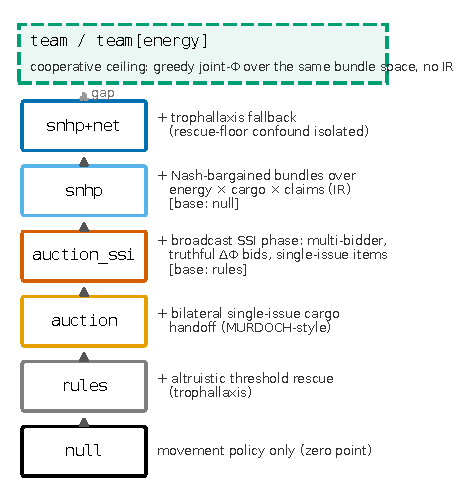
\includegraphics[width=\linewidth]{fig1_ladder.pdf}
\caption{The arm ladder: one mechanism per rung, null $\to$ rules $\to$
auction $\to$ auction\_ssi $\to$ snhp $\to$ snhp+net, with team /
team[energy] as the cooperative-ceiling rail. \texttt{[base: x]} tags mark
rungs whose base is not the previous rung (auction\_ssi = rules + SSI; snhp
= null + bundles).}
\label{fig:ladder}
\end{figure}

Bundles combine three issues --- energy, cargo, and sector/claim rights ---
in a discrete contract space ($7\times7\times2$ in the rich stage);
Figure~\ref{fig:bundle} shows one executed bundle. Bundle evaluation and
execution share one code path; evaluated $\Phi$ == executed $\Phi$ is
asserted on every deal. \texttt{auction\_ssi} shares every discipline with
the other rungs (same item magnitudes, same 1.1 clearing hysteresis, same
transaction cost, pause, cooldowns) and differs from \texttt{auction} by
exactly \{broadcast multi-bidder, energy-as-item, sequential rounds\}; an
item is exactly a $(q,0,0)$ or $(0,e,0)$ bundle, so the arm structurally
cannot logroll (asserted in code). Later rungs add hazard-priced risk
(\texttt{-hz}), career-value pricing (\texttt{-lv}, \texttt{-lvc}), company
walls, and a trust-gated joint tier (Section~\ref{sec:integrity}). The
\texttt{team} arm exists because hostile review showed a trivial selfless
control can dominate a bargaining arm; every bargaining claim faces both
the auctions below and the ceiling above.

\begin{figure}[t]
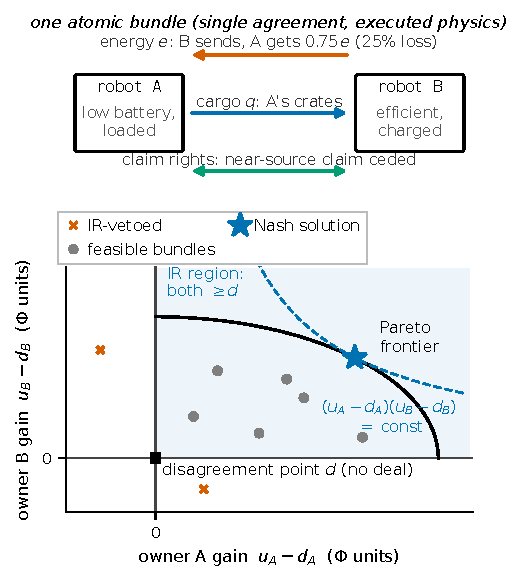
\includegraphics[width=\linewidth]{fig2_bundle.pdf}
\caption{One executed bundle between two robots: the three issue axes
(energy transfer with 25\% loss, cargo, claim rights) and the utility-gain
space with the IR region, disagreement point, Pareto frontier, and
Nash-product hyperbola. Geometry illustrative; the loss rate and issue
space are the spec constants of
Sections~\ref{sec:world}--\ref{sec:ladder}.}
\label{fig:bundle}
\end{figure}

\subsection{Metrics}\label{sec:metrics}

Primary: \textbf{delivered ore at the fixed 2500-tick horizon} --- never a
ratio whose denominator shrinks when robots die
(Section~\ref{sec:registration}). Strandings are first-class: every
headline is also reported as $\mathrm{score}_k = \mathrm{delivered} -
k\cdot\mathrm{stranded}$ at $k \in \{0, 2, 5\}$, after an audit showed the
agents internally price a stranded drone at 1.5 ore while the scoreboard
priced it at 0. Secondaries: energy efficiency metered to the last
delivery, lost cargo, deal counts, multi-issue fraction, per-deal capture.
Statistics: paired $t$ and Wilcoxon on 24 seeds (16 in later columns),
wins/$n$, Holm within families; makespan reported but not tested where
horizon censoring dominates.

\subsection{Registration protocol --- and the v1 failure as
method}\label{sec:registration}

The v1 headline claims failed hostile review: the efficiency metric
\emph{rewarded fleet death} (dead robots stop drawing charge; one run
stranded all 24 robots, delivered less than the auction, and scored ``a
5.8$\times$ win''); a trivial greedy joint-$\Phi$ control beat the
bargaining arm on every metric at every $\sigma$; and the single-issue
ablation struck zero deals --- the failure that became C1. SPEC v2 was
re-registered on 2026-07-14, \emph{before any v2 results}, with claims
C1--C3, the mean-preserving dial, the cooperative ceiling as a mandatory
arm, delivered-at-horizon as primary, and explicit WIN/PARTIAL/KILL
outcomes; every later extension (v3--v12, columns A--K, and review-response
columns R1/GB/SSI) was registered pre-run with its own kill condition. A
2026-07-15 replay review then found two physics artifacts that 22 automated
passes had missed --- a cargo trap whose rescue subsidized our own
mechanism by ${\sim}40\%$ of the then-current bargaining-vs-auction gap,
and temporally free deals; all columns were re-run, several verdicts shrank
or died, and Section~\ref{sec:results} reports post-correction numbers
(detail, including a charger livelock, in
Appendix~\ref{app:corrections}).

\section{Results}\label{sec:results}

All verdicts are read against their pre-registrations. Sweep sizes: v2.1
888 runs; v3 960; v4.0 1944; v4.1 544; v5 736; v6--v7 480; columns G--K 16
seeds/cell; R1 (384 runs, 64 seeds), GB (360), SSI (216) per the 2026-07-23
addendum, whose headline test is Wilcoxon ($p_w$).

\subsection{C1 --- bundling is necessary under individual
rationality}\label{sec:c1}

Registered prediction P1 (single-issue snhp arms strike 0 deals at every
$\sigma$) \textbf{holds as amended}. Energy-only trade is structurally
impossible: with 25\% transfer loss and selfish utilities the donor always
loses. Cargo-only trade exists solely as \emph{distress jettison}
(${\sim}0.5$ deals/run): a near-stranded loaded robot gains by shedding
load. Both are pinned as test invariants. In the full arms,
${\sim}$98--99\% of struck deals are multi-issue (per-run range 86--100\%;
HEAD-physics artifact \texttt{sweep\_v2.1\_head.json}). The cooperative
form did \textbf{not} survive the physics correction: on the HEAD re-pin
(R4), \texttt{team} beats \texttt{team[energy]} only at $\sigma{=}0.75$
($+1.62$, $p_w{=}.014$; elsewhere $-0.7$ to $+2.5$, n.s.) --- once deals
cost time, extra bundle dimensions stop paying at the cooperative ceiling.
The rebuttal of ``single-issue suffices'' rests on the structural IR half
of C1 alone; the pre-correction ``$+1.8$ to $+17.1$, significant at 4 of 5
$\sigma$'' figure is retired to the correction history.

C1 recursed one level up: in the column-K information market
(Section~\ref{sec:colk}), a map-sync whose net value to the buyer is
negative (bad news only) is IR-vetoed by construction; bad news trades only
when bundled with enough good news to clear the veto. Single-issue bad news
is unsellable; bundled truth trades.

\subsection{C2 --- sufficiency and the coordination gap}\label{sec:c2}

Every C2 comparison names its baseline: against the \textbf{bilateral
MURDOCH-style handoff auction} (\texttt{auction}) bargaining wins
delivered; against the \textbf{broadcast SSI auction}
(\texttt{auction\_ssi}) it does not --- a registered kill (below, and
Section~\ref{sec:kills}).

All harsh-world numbers are the HEAD-physics re-pin (R4, registered
2026-07-23; artifact \texttt{sweep\_v2.1\_head.json}, 888 runs; the
2026-07-14 artifact is history only). \texttt{snhp+net} beats
\texttt{auction} at every $\sigma$ ($+3.33$ to $+7.00$ delivered;
$p_w{\leq}.014$ at $\sigma \in \{0, 0.25, 0.5\}$, $p_w{=}.052$ at
$\sigma{=}0.75$, $p_w{=}.011$ at $\sigma{=}1.0$), with k2/k5 gaps larger
and significant at every $\sigma$ ($\sigma{=}0.5$ k5 $+25.96$,
$p_w{=}.0001$) --- the registered R4-C2 ordering, WIN
(Figure~\ref{fig:delivered}). The v2.1-era ceiling inversion (119.6 vs
105.9 at $\sigma{=}0$) survives only in survival form: under HEAD the
$\sigma{=}0$ delivered edge over \texttt{team} is $+1.62$ $[-0.27, +3.52]$
($p_w{=}.11$ at 24 seeds; $+1.77$, $p_w{=}.026$ at the 64-seed R1a re-pin),
carried by strandings (2.6 vs 4.1; k5 $+9.58$, $p_w{=}.0002$ at 64 seeds);
the hive wins delivered outright at $\sigma{\geq}0.75$ ($-15.46/-12.00$,
$p_w{\leq}.0002$). \texttt{snhp} beats \texttt{null} at every
$\sigma{\geq}0.25$ ($+23.0$ to $+31.0$, 23--24/24 seeds, $p_w{\leq}.0001$)
but \textbf{loses at $\sigma{=}0$} ($-6.29$ $[-8.61, -3.97]$,
$p_w{=}.0001$, 2/24): twin fleets have no gains from trade, so bargaining
is pure overhead --- as theory demands. Corrected honest negatives: at
$\sigma{\leq}0.5$ pure \texttt{snhp} still never beats the auction on
delivered (the low-$\sigma$ win requires the rescue floor; at
$\sigma{=}0.75$ it now does, $+7.21$, $p_w{=}.0089$); the pre-correction
``net hurts at $\sigma{=}0.75$'' tax (99.3 vs 90.4) was a physics artifact
--- under HEAD it vanishes (snhp $-$ snhp+net $= +1.58$, n.s.) and the net
helps significantly at every other $\sigma$.

\begin{figure*}[t]
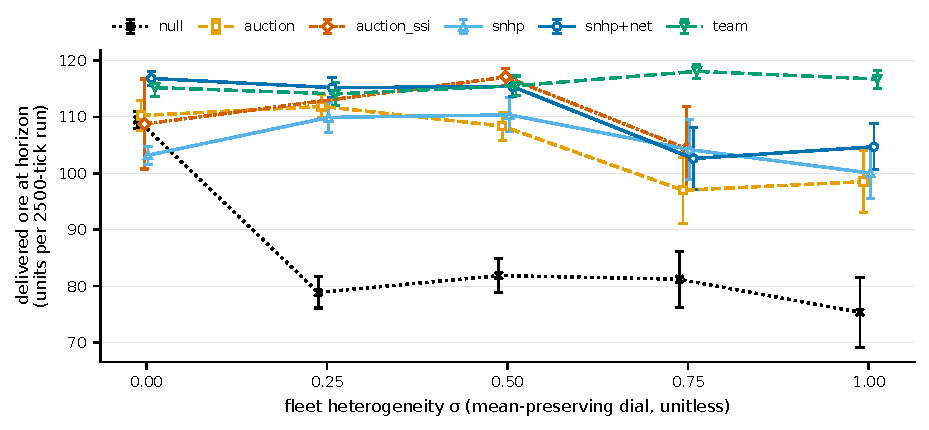
\includegraphics[width=\linewidth]{fig3_delivered_sigma.pdf}
\caption{Delivered-at-horizon vs $\sigma$ (mean $\pm$ 95\% CI, 24
seeds/cell) for null, auction, auction\_ssi, snhp, snhp+net, and team on
the HEAD-physics v2.1 grid (\texttt{sweep\_v2.1\_head.json}); the
auction\_ssi series is from \texttt{sweep\_v4\_SSI.json} ($\sigma \in \{0,
0.5, 0.75\}$ only).}
\label{fig:delivered}
\end{figure*}

The \textbf{coordination gap} (team $-$ snhp on delivered; registered as
``price of selfishness,'' renamed here) is real at every $\sigma$ and grows
past mid-$\sigma$: $12.0 \to 4.2 \to 5.2 \to 13.9 \to 16.7$ as $\sigma$
goes $0{\to}1$ (HEAD re-pin; all $p_w{\leq}.048$). Registered prediction P3
(that it \emph{shrinks} with $\sigma$) remains \textbf{refuted}: the gap
dips at mid-$\sigma$, then grows. The gap is not the price of anarchy
\cite{koutsoupias1999worstcase}: PoA bounds worst-case \emph{equilibrium}
welfare against the \emph{optimum}, whereas ours is the measured difference
between one IR mechanism and a greedy joint-utility heuristic --- neither
an equilibrium notion nor an optimum bound (the ceiling itself is
non-optimal, Section~\ref{sec:limitations}). It is an empirical gap for
this world and ladder, not a named theoretical quantity.

\begin{figure}[t]
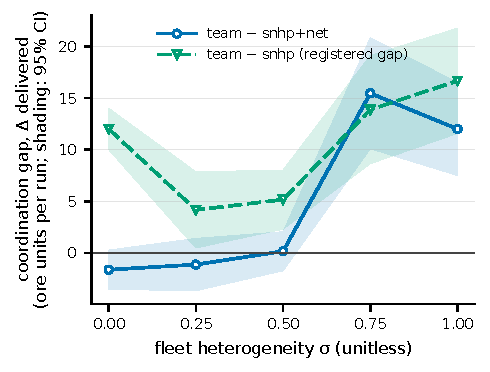
\includegraphics[width=\linewidth]{fig4_gap.pdf}
\caption{The coordination gap vs $\sigma$: paired $\Delta$ delivered with
95\% CI bands for \emph{both} definitions --- team $-$ snhp (the registered
gap, formerly ``price of selfishness''; this is the curve the text's $12.0
\to 4.2 \to 5.2 \to 13.9 \to 16.7$ numbers refer to) and team $-$ snhp+net
(the survival-form comparison against the safety-netted arm). The two
diverge sharply at $\sigma \leq 0.5$, where the rescue floor does most of
its work.}
\label{fig:gap}
\end{figure}

The physics correction shrank but did not kill the bilateral comparison on
the rich stage: snhp-hz $+3.4$ ($p{=}.005$, was $+9.6$ --- ${\sim}40\%$ of
the old gap was the pad subsidy), positive at every counterparty-noise
level ($+0.8$..$+4.1$, $p{\leq}.024$; the v5 noise dial found no crossover
--- the true-loss veto turns estimation error into failed proposals, not
bad deals); on k-scores only the safety-net arm survives (snhp+net vs
auction $+4.5$ delivered, $+20.4$ at $k{=}5$, both significant). The
``market beats the hive'' claim, re-pinned at 64 seeds (R1a, WIN): $+1.77$
delivered $[+0.32, +3.21]$, $p_w{=}.026$, strandings 2.27 vs 3.83, k5
$+9.58$, $p_w{=}.0002$; the seeds-0..15 subset reproduces the previously
unversioned 16-seed numbers essentially exactly ($+2.12$, $p_w{=}.041$). On
richer stages the hive wins at every $k$. The scoped law: \emph{the
safety-netted market beats central planning when survival is the binding
constraint; the hive wins when logistics are.}

\paragraph{Two-geometry replication (R2/column GB: WIN).} On geometry B ---
sources at Manhattan 32/24 in opposite quadrants (no cheap 16-hop source,
no 40-hop death-march), refinery mid-edge, mid-field charger, non-mirrored
--- (snhp+net $-$ auction) delivered is positive at every $\sigma$: $+6.42$
($p_w{=}.0002$) at $\sigma{=}0$, $+3.83$ ($p_w{=}.0038$, 18/24) at
$\sigma{=}0.5$, $+4.42$ ($p_w{=}.0007$, 19/24) at $\sigma{=}1.0$, with no
k2 reversal ($\sigma{=}0.5$ k5 $+26.96$, $p_w{=}.0001$). The ladder
ordering replicates descriptively. Nuance, reported as registered: on B the
hive is \emph{not} edged on raw delivered at $\sigma{=}0$ (118.8 vs 119.5,
at the 120 ceiling) --- but team strands 9.17 vs 0.96, so the net dominates
every k-score; the survival form of the law holds on both maps. The
bilateral comparison in C2 is a two-geometry result.

\paragraph{The strong-market test (R3/column SSI: KILL FIRED).} The
registered prediction that snhp+net out-delivers SSI at $\sigma{\geq}0.5$
died in its strong form: auction\_ssi \emph{significantly beats} the
bargaining arm on delivered at $\sigma{=}0.5$ ($-1.75$ $[-3.48, -0.02]$,
$p_w{=}.038$; $\sigma{=}0.75$ $-1.75$, n.s.). The SSI market pays in
strandings: snhp+net wins $\mathrm{score}_{k=5}$ at $\sigma{=}0.75$
($+12.42$, $p_w{=}.027$) and dominates the k-scores at the $\sigma{=}0$
sanity cell (k2 $+19.92$, k5 $+37.67$, both $p_w{\leq}.0001$). The kill was
earned against a real opponent: auction\_ssi beats the bilateral auction by
$+8.75$ ($p_w{=}.0001$) at $\sigma{=}0.5$ and $+7.38$ ($p_w{=}.045$) at
$\sigma{=}0.75$. The honest statement of C2: \emph{against a strong market
baseline, bargaining buys survival, not throughput} --- the fourth time a
strengthened market matched or beat bargaining on raw output while losing
on fleet survival (v3 hazard pricing, v9 career pricing, the v11 moving
field, now SSI).

\subsection{C3 --- heterogeneity scaling}\label{sec:c3}

Registered prediction P4 (snhp $-$ bilateral auction grows monotonically in
$\sigma$) is \textbf{partial} and survives the HEAD re-pin (R4-C3, WIN):
$-7.0 \to -2.0 \to +2.0 \to +7.2 \to +1.5$ delivered across $\sigma \in
\{0, 0.25, 0.5, 0.75, 1.0\}$ (\texttt{sweep\_v2.1\_head.json}) ---
point-estimate monotone over $\sigma{=}0{\to}0.75$ (a 14.3-unit swing,
${\sim}60\%$ smaller than the pre-correction 36.6; $+7.21$ at
$\sigma{=}0.75$, $p_w{=}.0089$), saturating or breaking at $\sigma{=}1.0$.
The break is unexplained (candidates: robots no deal can salvage; charger
binding); we do not claim full monotonicity. The $\sigma{=}0$ end is now
significantly negative ($-7.04$, $p_w{=}.0001$): twin fleets have nothing
to trade, so bargaining is overhead on this world; in the two-company v4
world at $\sigma{=}0$ all mechanisms statistically tie \texttt{null}
(post-correction) --- the same no-heterogeneity-no-gains prediction at each
world's cost structure. The strongest effect is the two-company v4 world:
snhp beats auction $+15.5/+15.0$ delivered at $\sigma{=}0.5/1.0$
($p{<}0.001$, 22--23/24 seeds) pre-correction; $+14.1$ ($p{<}.001$) on the
corrected v4 preset. Geometry scoping: the gap's \emph{sign} at
$\sigma{\geq}0.5$ replicates on geometry B (Section~\ref{sec:c2}), but the
five-point gradient is geometry-A only --- on B the gap is already
significant at $\sigma{=}0$ ($+6.42$, $p_w{=}.0002$; B's distances keep
charging economics binding even for twin fleets), so the
growth-with-$\sigma$ shape remains a geometry-A result.

\subsection{Killed claims (reported as registered)}\label{sec:kills}

The registered kill conditions fired repeatedly; the decision-relevant
deaths are listed inline.

\begin{itemize}
\item \textbf{``Beats the market lineage'' (R3/column SSI): KILL FIRED, the
strong form.} The broadcast SSI baseline significantly out-delivers
snhp+net at $\sigma{=}0.5$ ($-1.75$, $p_w{=}.038$) and never loses on
delivered at $\sigma{\geq}0.5$, while snhp+net keeps the survival-adjusted
scores (k5 $+12.42$, $p_w{=}.027$ at $\sigma{=}0.75$). Registered
consequence, applied without spin: every C2 delivered claim names its
baseline --- the bilateral MURDOCH-style handoff --- and no general ``beats
the market lineage'' language survives (numbers in
Section~\ref{sec:c2}). Structural note: auction\_ssi is single-issue by
construction and cooperative (truthful $\Delta\Phi$ bids, no payments); its
awards are not IR (the losing side eats a negative $\Delta\Phi$ whenever
$1.1\times|\mathrm{loss}| < \mathrm{gain}$), so C1 --- single-issue
\emph{IR} trade is infeasible --- stands untouched.
\item \textbf{Hazard-priced risk as a substitute for the rescue floor (v3):
killed.} Both registered kill triggers fired (snhp-hz $\leq$ snhp at
$\sigma{=}0.25$, $-8.4$, $p{=}0.034$; the net still added $+22.8/+25.1$
delivered at $\sigma{\leq}0.25$). The surviving v3 ``regime law'' (risk
pricing wins when risk is heterogeneous) then \textbf{died under corrected
physics}: its crossing was largely the pad-subsidy artifact (best remaining
edge $+3.6$, $p{=}.17$, with 15--21 strandings vs the net's 2--7).
\item \textbf{Career-value drone pricing (v9/column H): kill fired.}
Pricing drones at their remaining mining career made late-game drones
disposable (delivered $-16.5$, $p{=}.023$; stranded $+7.3$, $p{=}.001$ vs
flat pricing). With a capital floor it set the fastest selfish makespan
recorded (688) and tied the net on delivered (239.6) --- but still lost
$\mathrm{score}_{k=5}$ by $-36$ ($p{=}.001$). Three attempts to replace the
rescue floor with a smarter market (v3, v6, v9) died on pre-registered
criteria: \emph{the safety net's edge is institutional, not a pricing
bug.}
\item \textbf{The density theory (v8/column G): killed as stated.} ``Dense
fields favor auction, sparse favor bargaining'' was replaced by a hump:
snhp+net $-$ auction $= +4.1$ (grid 24) $\to +4.5$ (32) $\to +7.3$ (48)
$\to -2.7$ (64); see Figure~\ref{fig:hump}. A market needs enough logistics
friction to be worth paying for and enough meeting density to convene.
Single-geometry; scoped accordingly.
\item \textbf{``Cooperation is 43\% faster'': died under corrected
physics.} Once deals cost time, the joint tier's speed edge is ${\sim}9\%$
n.s.; the dividend moved to survival (gated fleets end 1.06 stranded vs the
veto tier's 15.31).
\end{itemize}

\begin{figure}[t]
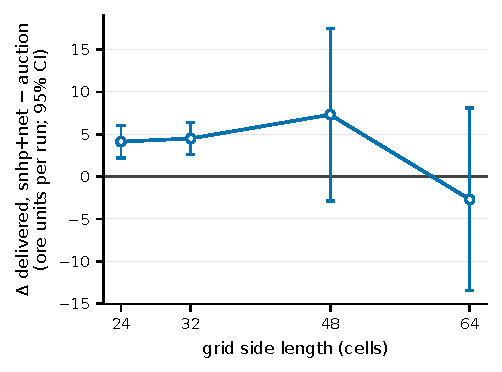
\includegraphics[width=\linewidth]{fig5_hump.pdf}
\caption{The v8 hump (single geometry; v5 preset, $\sigma{=}0.5$, 16
seeds/cell): (snhp+net $-$ auction) delivered vs grid side 24/32/48/64,
paired $\Delta$ with 95\% CI whiskers ($+4.12$ / $+4.50$ / $+7.31$ /
$-2.69$).}
\label{fig:hump}
\end{figure}

\subsection{Deception and self-knowledge error: scoping
note}\label{sec:integrity}

The program's integrity results belong to a companion paper; here they are
only scoped. The v6.0 registered kill fired informatively: Nash-IR
bargaining with a true-loss veto is intrinsically deception-tolerant ---
lying barely pays because every executed deal clears both true disagreement
points; exploitation requires the trusting joint tier, where attestation
gating drops the liar advantage to statistical zero. v7 showed
self-knowledge error (a miscalibrated gauge) leaves output flat while
silently signing deals at negative true surplus. The relevance to C2: the
bargaining tier's IR guarantee is exactly as good as each robot's knowledge
of its own state, and information quality was a treated variable, not an
assumption.

\subsection{Column J --- the moving field inverts a
headline}\label{sec:colj}

On static fields, perfect field information was never load-bearing (column
I: oracle $-$ belief $= +0.2$ delivered, n.s.; the registered whole-column
kill fired). Column J removed the crutches: seeded arrivals nobody knows
about, departures that leave ghosts on stale maps, contested unmirrored
ground.

\begin{itemize}
\item \textbf{P16a failed as registered}: oracle $-$ belief on delivered is
$+11.4$, directional but n.s.\ at 16 seeds ($p{=}.15$). The
\emph{significant} information-value channel is the books: belief-mode
signs $+7.0$ more truly-harmful deals per run ($p{=}.0004$).
\item \textbf{P16b inverted, significantly}: the auction, with
substantially staler maps (358.4 vs 262.8 ticks at the 64-seed re-pin,
$p_w{=}.029$; 16-seed: 305 vs 190), captures \emph{more} of the newly
arrived stock: $+8.98$ $[+0.44, +17.52]$, $p_w{=}.022$ (42.7 vs 33.7
units/run) at 64 seeds (R1c, WIN); 16-seed original 46.2 vs 32.4,
$p{=}.03$ --- shrank from $+13.8$ but holds
(Figure~\ref{fig:inversion}). Discovery needs physical coverage: the deal
economy converges robots onto known-profitable loops, while the auction's
inefficient wandering is accidental exploration.
\item \textbf{Exploratory, flagged post-hoc}: on the moving contested field
the auction out-delivers every coordination arm on raw gold (snhp+net
$-12.6$, $p{=}.044$ at 16 seeds; $+10.19$, $p_w{=}.011$ at 64 seeds ---
reported but never registered, so it stays post-hoc) while k2/k5 remain a
wash ($+7.1$ n.s.\ / $+2.5$ n.s.: the auction pays its gold edge in dead
drones). The discovery gap explains the delivered gap almost exactly (13.8
arrival-units $\approx$ 12.6 delivered at 16 seeds). \textbf{Optimization
buys blindness to novelty}: the bargaining advantage is a known-field
phenomenon; novelty-rich worlds reward coverage over coordination.
\end{itemize}

\begin{figure}[t]
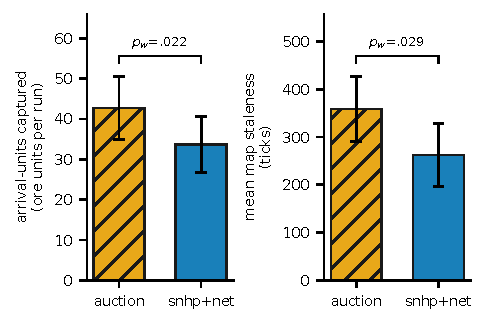
\includegraphics[width=\linewidth]{fig6_inversion.pdf}
\caption{The column-J inversion at the 64-seed re-pin (R1c cells of
\texttt{sweep\_v4\_R1.json}; moving + contested + belief-mode, no scouting
or map market): arrival-units captured (42.70 vs 33.72, $p_w{=}.022$) and
mean map staleness (358.4 vs 262.8 ticks, $p_w{=}.029$), auction vs
snhp+net. The arm with fresher maps captures \emph{less} of the new stock
--- freshness $\neq$ discovery.}
\label{fig:inversion}
\end{figure}

\subsection{Column K --- scouting fixes discovery; the map market fixes the
books}\label{sec:colk}

Column K priced the unknown. The discovery deficit died to \emph{policy},
not markets: two scouts per company erased the auction's explorer edge
(arrivals gap $-13.8$, $p{=}.03 \to -3.4$, n.s.; delivered 284.1 vs 286.6)
and made the oracle redundant (282.8 vs 284.1 --- with patrols, information
is free again). A Nash-priced map market (40 executed syncs/run) added
nothing to discovery ($-0.7$, $p{=}1.0$) but \textbf{cut poisoned deals
${\sim}30\%$} --- re-pinned at 64 seeds (R1b, WIN): \textbf{5.00 $\to$ 3.53
($-29\%$), $p_w{=}.0007$} (16-seed original: 5.38 $\to$ 3.75, $p{=}.04$),
with delivered a descriptive wash ($+4.53$, $p_w{=}.46$): \emph{traded
information's product is audit integrity, not output}
(Figure~\ref{fig:poisoned}). The registered bad-news trap (P17c) confirmed
structurally: bad-news-only syncs are IR-vetoed; bundled truth trades
(Section~\ref{sec:c1}). Prospecting claims produced measurable patrol
differentiation (staleness 22.7 vs 25.4 inside vs outside own claims) with
zero output effect at this scale.

\begin{figure}[t]
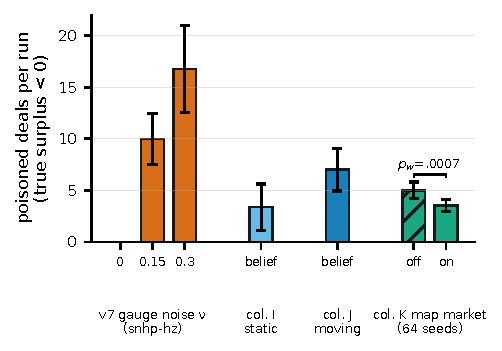
\includegraphics[width=\linewidth]{fig7_poisoned.pdf}
\caption{Poisoned deals per run (executed at negative true surplus for an
honest party) across the program's error sources: v7 gauge noise ($\nu \in
\{0, 0.15, 0.3\}$; snhp-hz, no margin, 32 seeds), column I static-field
beliefs (16 seeds), column J moving-field beliefs (16 seeds), and column K
map market off/on at the 64-seed re-pin (5.00 $\to$ 3.53,
$\Delta{=}+1.47$ $[+0.69, +2.24]$, $p_w{=}.0007$). Output stays flat in
every condition; only the books move.}
\label{fig:poisoned}
\end{figure}

\section{Discussion}\label{sec:discussion}

\textbf{Mechanism choice for cross-organization fleets is regime-dependent,
and the regimes are now mapped.} Bundling is necessary for any IR trade
(C1, structural). Bargaining plus an unconditional rescue floor
out-delivers a bilateral handoff auction on two geometries and, on
survival-bound worlds, edges past the cooperative ceiling (C2); against the
broadcast SSI lineage its edge is survival-priced, not throughput ---
continuous with the standing result that the safety net's value is
institutional. The advantage needs heterogeneity (C3), mid-range logistics
friction with enough encounter density (the v8 hump, single-geometry), and
a \emph{known} field (column J). Where those fail, simpler mechanisms win
honestly: coverage beats coordination on novelty-rich ground, SSI
competition matches bargained throughput, and central planning wins when
logistics rather than survival bind. For an operator: choose by what binds
--- throughput (a strong auction suffices), fleet survival (bargaining + a
rescue floor), or discovery (coverage/scouting policy).

\textbf{The border result is the deployment-relevant one.} Two firms
bargaining at their boundary statistically match a full merger (team 118.6
vs twofirm 117.6, n.s., corrected physics); selfless cross-company
transfers are net-harmful; posted-price infrastructure tolls collapse
against a bargaining fleet (peak toll revenue $-63\%$, 72.1 $\to$ 26.8).
You do not need to merge fleets --- you need a bargaining layer at the
boundary, with IR keeping the border priced rather than closed or
exploited.

\textbf{The integrity thread is deliberately excluded.} Across four error
sources --- lies (v6), gauge miscalibration (v7), stale maps (v10), a
moving field (v11) --- output stays flat while individual books silently
bleed, and column K's map market heals books, not output. That finding and
its settlement-infrastructure implications form the companion paper.

\section{Limitations}\label{sec:limitations}

This is a mechanism benchmark; hardware grounding is future work.

\begin{itemize}
\item \textbf{Scale}: $N{=}24$ (16--24 seeds per cell) is a multi-robot
economy, not a swarm; by {\c{S}}ahin's criteria \cite{sahin2005swarm} no
swarm claim is made or licensed.
\item \textbf{Deterministic gridworld}: physical grounding here means
world-dynamics-derived utilities, not hardware --- there are no kinematics,
collisions, sensor/actuation noise, or comms dropout, and noise-free
simulation results are presumed non-transferable across the reality gap
\cite{jakobi1995noise,jakobi1997radical} until shown otherwise.
\item \textbf{Full-information utilities}: robots know their own $\Phi$
exactly (v7 perturbs one input); counterparty utilities are estimated only
in v5+. Strategic information revelation and opponent learning are touched
only through the registered lie and noise channels.
\item \textbf{Deal-space abstraction}: energy transfer (lossy, minutes),
cargo handoff (precision docking), and claim swaps (instant, free) have
very different hardware time constants and failure modes; treating them as
commensurable in one atomic bundle needs justification before any hardware
claim.
\item \textbf{Static-vs-moving scoping}: the headline bargaining advantages
hold on static or slowly-changing fields; column J shows the ordering can
invert under non-stationarity. Claims are scoped accordingly.
\item \textbf{Statistical power and geometry}: the three previously fragile
headline numbers were re-pinned at 64 seeds (R1, all WIN) and the C2
bilateral comparison replicates on a second geometry (R2); but 16-seed
columns still leave directional results unresolved (P16a: $+11.4$,
$p{=}.15$), the v8 hump and later-column findings remain single-geometry,
and the C3 $\sigma$-gradient shape is geometry-A only. Exploratory findings
are flagged and must not be cited as registered.
\item \textbf{Mechanism instantiations}: the auction lineage has two rungs
(bilateral MURDOCH-style and broadcast SSI \cite{koenig2006ssi}), but
combinatorial variants are untested; the cooperative ceiling is greedy
joint-$\Phi$, not an optimal planner, so the coordination gap is measured
against a heuristic, not an optimum.
\end{itemize}

\section{Reproducibility}\label{sec:repro}

The pipeline is deterministic and seed-pinned. Code and artifacts are
released as a self-contained repository at
\path{github.com/ryuxik/bundling-or-silence} (public at publication;
Apache-2.0;
the 174-test suite passes on a clean clone; source hashes in
\path{PROVENANCE.md}). The world, arms, and runner are \texttt{world.py},
\texttt{arms.py}, \texttt{run.py}; every column is regenerated by
\texttt{run.py --column} with column id \texttt{A}..\texttt{K},
\texttt{R1}, \texttt{GB}, or \texttt{SSI}, then \texttt{run.py --analyze}
on the sweep JSON (v2.1/v3 via \texttt{run.py} directly; review-response
numbers print from the committed \path{repin_report} path, not notebooks).
Sweep artifacts (per-run rows with seeds, arm configs, event logs) are
committed under \path{research/swarm/results/} (e.g.\
\path{sweep_v2.1.json}, 888 runs; \path{sweep_J.json} /
\path{sweep_K.json}, 16 seeds/cell; \path{sweep_v4_R1.json}, 384 runs at
64 seeds; \path{sweep_v4_GB.json}, 360 runs; \path{sweep_v4_SSI.json}, 216
runs). The test suite (\texttt{pytest} \path{test_swarm.py}, 174 tests
green as of the addendum) pins the structural claims (C1 zero-deal
invariants, $\sigma$ mean-preservation, evaluated==executed dynamics,
attested-all $\equiv$ honest-all bit-identity, the auction\_ssi
single-issue assertion) and regression-pins the corrected physics.
Disclosure: the bargaining primitives
(\path{generate_contract_space}, \path{filter_pareto_frontier},
\path{find_nash_bargaining_solution}) are the authors' deployed
production negotiation engine's code, reused unmodified --- deliberately,
so the benchmark exercises the code path that ships. Pre-registrations,
amendments, and fired kills are timestamped in \texttt{SPEC.md} and
\path{SPEC-ADDENDUM-2026-07-23.md} (verdicts appended after runs;
registrations never edited); the hostile v1 review, the standards brief,
and the 2026-07-23 referee review are in \texttt{review/}.

\appendix

\section{The physics corrections (detail)}\label{app:corrections}

The 2026-07-15 replay review found: (1) a \emph{pad-strand cargo trap} ---
a robot arriving at its target facility could strand on the arrival step
and hold its cargo forever; rescue-capable arms ransomed that cargo back at
94--100\% vs ${\sim}64\%$ for auction/rules, a differential subsidy to our
own mechanism worth ${\sim}40\%$ of the then-current bargaining-vs-auction
gap; and (2) \emph{temporally free deals} --- robots kept driving
mid-exchange. Fixes: facilities unload on arrival (same tick); every
executed exchange immobilizes both parties for DEAL\_PAUSE${=}3$ ticks. A
third audit finding motivated the k-score policy: the scoreboard priced a
dead drone at $k{=}0$ while the agents priced it at 1.5 ore internally, so
every headline is reported at $k \in \{0, 2, 5\}$. Separately, a 22-agent
pre-merge review found a \emph{charger livelock} in the v7 column (the
queue-release threshold read believed battery while the cap uses true
battery, parking robots with gauge bias $< -0.05$ at chargers forever;
reproduced 3$\times$) plus a second unintended perturbation channel; both
were fixed, regression-pinned, and columns D/E/F re-run, with pre-fix
numbers struck in the results file.

% Bibliography-only entries (present in the markdown reference list but not
% cited in-text there either): keep the two lists identical.
\nocite{brambilla2013swarm,hamann2018swarm}

\bibliographystyle{ACM-Reference-Format}
\bibliography{refs}

\end{document}
